\documentclass[12pt,a4paper]{article}
\usepackage{amsmath}
\usepackage{amsfonts}
\usepackage{amssymb}
\usepackage{graphicx}
\usepackage{secdot}
\usepackage{multirow}
\usepackage[left=2cm,right=2cm,top=2cm,bottom=2cm]{geometry}

\title{{Experiment - 3\\Force due to Jet impact}}
\author{Arka Pramanick, AE21B007\\ Department of Aerospace Engineering\\ IIT Madras\\[3ex] Instructor:\\ \large Professor Dr. R. Sriram}

\date{13 February, 2023}


\begin{document}
\maketitle

\hline

\section{Aim :}
To calculate reaction forces due to change in momentum of a fluid flow as jet of water strikes the plate. 
\section{Apparatus :}
Required apparatus for performing this experiment are:
\begin{itemize}
    \item Plates of different angles(90$^{\circ}$, 120$^{\circ}$ and 180$^{\circ}$)
    \item Weights
    \item Stopwatch 
    \item Jet Apparatus(Having nozzle of diameter 0.008m)
\end{itemize}

\section{Theory :}


Volume flow rate(Q) =\begin{equation}
    Q = A u
\end{equation} $A u$\\
Mass flow rate = \begin{equation} Q_m =\rho A u    
\end{equation}
Applying conservation of momentum in figure :\\
\underline{X axis} : Net momentum = 0 \\
$\underline{Y axis}$ : Outflux = -$Q_mu$ ($\sin {\theta}$) \hspace{2mm} Influx = $Q_mu$ \\Rate of change in momentum = -$Q_m u\sin {\theta}$- $Q_mu = -Q_mu$(1+$\sin{\theta}$)\\
Using equation(1) :\\
\begin{equation}
F_y = \rho A u^{2}(1 + \sin{\theta})\\
\end{equation}
$\rho$ : Density of fluid.\\
$A$ : Cross section area of the nozzle.\\
$u$ : Velocity of water leaving nozzle.\\
$\theta = \alpha - \frac{\pi}{2}$; $\alpha$ is the deflection angle.





\section{Procedure :}
\begin{enumerate}
    \item Mass of fixed mass is first placed on a weight pan.
    \item It is checked whether the datum line is on weight panel is on the same level of gauge.
    \item Valve is opened slowly and stopwatch is started.
    \item Flow rate is measured by stopping timer after measuring time it take to accumulate a particular volume of water.
    \item Process is repeated on adding additional mass.
    \item Whole test is repeated for three different deflection angle.
\end{enumerate}






\section{Observation :}

\subsection{Force due to jet impact on a deflector of turn angle $120^{\circ}$}
\begin{table}[ht]


\begin{flushleft}
\begin{tabular}{ |c|c|c|c|c|c|c|c|c| } 
\hline

 \multirow{2}{*}{Test No.} & \multicolumn{8}{c|}{Angle deflector = $120^{\circ}$ } \\ \cline{2-9}
                           & Mass(g)& Weight(N) & Volume(L) & Time(s) & Q($\times10 ^{-3}$) & Velocity(u) & $u^2$ & Force(N)\\ \hline
 1                         & 50 & 0.49 & 3 & 21.5 & 0.140 & 2.776 & 7.706 & 0.583  \\ \hline
 2                         & 100 & 0.98 & 3 & 16 & 0.188 & 3.730 & 13.914 & 1.052 \\ \hline
 3                         & 150 & 1.47 & 3 & 12.92 & 0.232 & 4.619 & 21.339 & 1.607\\ \hline
 4                         & 200 & 1.96 & 4 & 16.37 & 0.244 & 4.854 & 23.564 & 1.678\\ \hline
 5                         & 250 & 2.45 & 4 & 15.035 & 0.266 & 5.292 & 28.004 & 2.112 \\ \hline
 6                         & 300 & 2.94 & 4 & 13.14 & 0.304 & 6.056 & 36.677 & 2.762 \\ \hline
 7                         & 350 & 3.43 & 4 & 12.295 & 0.325 & 6.466 & 41.805 & 3.152 \\ \hline
 8                         & 400 & 3.92 & 4 & 10.665 & 0.375 & 7.460 & 55.657 & 4.196 \\ \hline
\end{tabular}
\end{flushleft}
\end{table}


\begin{figure}[!ht]
	\begin{center}
		\framebox{
			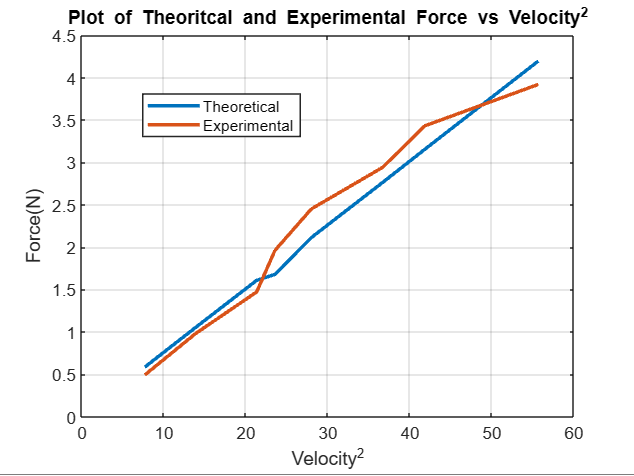
\includegraphics[scale=0.7]{ls 3.1.png}
		}
	\end{center}
	\caption{Theoretical and Experimental Pressure vs $Velocity^{2}$ for Angle delector = $90 ^{\circ}$}
\end{figure}

\newpage
\subsection{Force due to jet impact on a deflector of turn angle $90^{\circ}$}
\begin{table}[ht]


\begin{flushleft}
\begin{tabular}{ |c|c|c|c|c|c|c|c|c| } 
\hline

 \multirow{2}{*}{Test No.} & \multicolumn{8}{c|}{Angle deflector = $90^{\circ}$ } \\ \cline{2-9}
                           & Mass(g)& Weight(N) & Volume(L) & Time(s) & Q($\times10 ^{-3}$) & Velocity(u) & $u^2$ & Force(N)\\ \hline
 1                         & 50 & 0.49 & 1 & 6.38 & 0.157 & 2.785 & 7.757 & 0.437  \\ \hline
 2                         & 100 & 0.98 & 1 & 4.59 & 0.218 & 4.334 & 18.786 & 0.945 \\ \hline
 3                         & 150 & 1.47 & 1 & 3.56 & 0.280 & 5.570 & 31.030 & 1.560\\ \hline
 4                         & 200 & 1.96 & 1 & 3.25 & 0.308 & 6.121 & 37.471 & 1.885\\ \hline
 5                         & 250 & 2.45 & 6 & 17.46 & 0.344 & 6.837 & 46.738 & 2.352 \\ \hline
 6                         & 300 & 2.94 & 6 & 15.95 & 0.376 & 7.480 & 55.955 & 2.812 \\ \hline
 7                         & 350 & 3.43 & 6 & 14.57 & 0.412 & 8.193 & 67.119 & 3.376 \\ \hline
 8                         & 400 & 3.92 & 6 & 13.88 & 0.432 & 8.600 & 73.958 & 3.715 \\ \hline
\end{tabular}
\end{flushleft}
\end{table}
\begin{figure}[!ht]
	\begin{center}
		\framebox{
			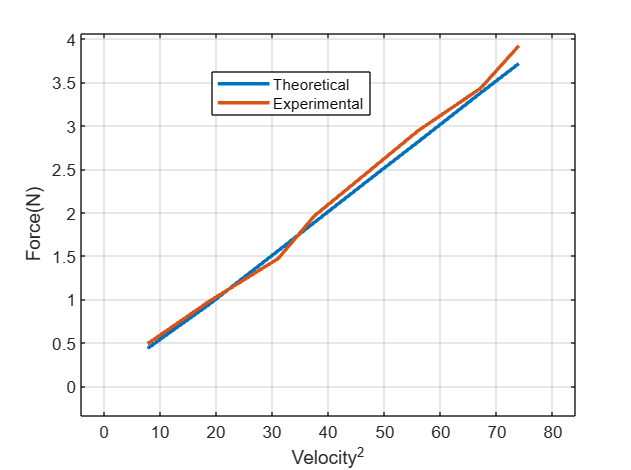
\includegraphics[scale=0.7]{ls 3.2.png}
		}
	\end{center}
	\caption{Theoretical and Experimental Pressure vs $Velocity^{2}$ for Angle delector = $90 ^{\circ}$}
\end{figure}

\newpage
\subsection{Force due to jet impact on a deflector of turn angle $180^{\circ}$}
\begin{table}[ht]


\begin{flushleft}
\begin{tabular}{ |c|c|c|c|c|c|c|c|c| } 
\hline

 \multirow{2}{*}{Test No.} & \multicolumn{8}{c|}{Angle deflector = $180^{\circ}$ } \\ \cline{2-9}
                           & Mass(g)& Weight(N) & Volume(L) & Time(s) & Q($\times10 ^{-3}$) & Velocity(u) & $u^2$ & Force(N)\\ \hline
 1                         & 50 & 0.49 & 3 & 25.47 & 0.118 & 2.348 & 5.513 & 0.554  \\ \hline
 2                         & 100 & 0.98 & 3 & 18.33 & 0.164 & 3.263 & 10.645 & 1.070 \\ \hline
 3                         & 150 & 1.47 & 4 & 18.57 & 0.215 & 4.277 & 18.295 & 1.839\\ \hline
 4                         & 200 & 1.96 & 5 & 20.56 & 0.243 & 4.834 & 23.370 & 2.349\\ \hline
 5                         & 250 & 2.45 & 5 & 18.69 & 0.268 & 5.322 & 28.326 & 2.853 \\ \hline
 6                         & 300 & 2.94 & 3 & 11.01 & 0.272 & 5.411 & 29.282 & 2.944 \\ \hline
 7                         & 350 & 3.43 & 3 & 10.69 & 0.281 & 5.583 & 31.171 & 3.138 \\ \hline
 8                         & 400 & 3.92 & 3 & 9.93 & 0.302 & 6.010 & 36.125 & 3.630 \\ \hline
\end{tabular}
\end{flushleft}
\end{table}
\begin{figure}[!ht]
	\begin{center}
		\framebox{
			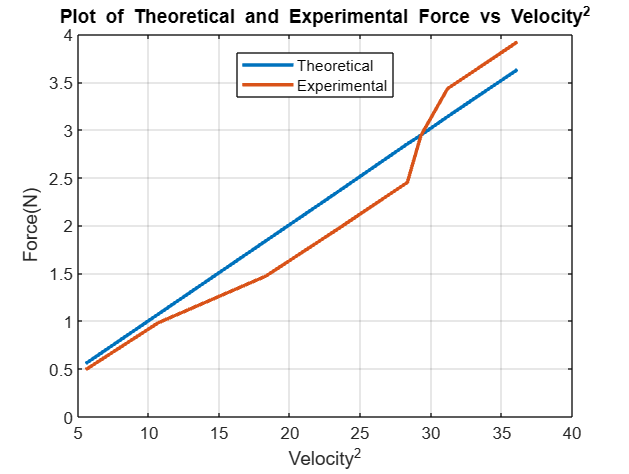
\includegraphics[scale=0.7]{ls3.3.png}
		}
	\end{center}
	\caption{Theoretical and Experimental Pressure vs $Velocity^{2}$ for Angle delector = $180 ^{\circ}$}
\end{figure}



\newpage

\section{Calculations :}
Calculations are shown for angle deflector = $120^{\circ}$ and Test No. 1 :\\
From experimental set up we know : \\
Area of nozzle(A) = $\frac{\pi \times (0.008)^{2}}{4}$;
Mass = 50g ; Volume of fluid(We took water as fluid for the experiment.) = 3L ; Time taken(t)=21.5s ;\\ $\alpha = 120 ^{\circ}$ $\implies $ $\theta = 30^{\circ}$ \\
Volume flow rate(Q) = $\frac{3 \times 10^{-3}}{21.5}$ = 0.140 $\times 10^{-3}$ $\frac{m^{3}}{s}$\\
From equation (1) : Velocity = $\frac{Q}{A}$ = 2.776 $\frac{m}{s}$\\
Force = $\rho Q u(1 + sin\theta) = 1000 \times 0.140 \times 10 ^{-3} \times 2.776 \times 1.5 $
      = 0.554 N
Theoretical force = 0.554N \\
Experimental force = 0.49 N \\
$\%$ error in force = 11.55 $\%$ \\





\section{Sources of Error:}
\begin{itemize}
    \item Error in measuring flow rate.
    \item Parallex error in checking datum line on weight pan is on the same level of gauge.
    \item Error due to environmental effect like temperature,pressure change.
    \item Instrumental error.
\end{itemize}



\section{Conclusion :}
\begin{itemize}
    \item Force due to jet impact is almost directly proportional to Velocity$^{2}$ 
    \item Experimental pressure somewhat deflects from Theoretical pressure.
    \item Reaction force is developed as jet of water strikes the plate.
    \item For a particular angle deflector flow rate and velocity increases as weight increases. 
\end{itemize}
\end{document}